\chapter{Identificação de Subsistemas}
\label{sec-subsistemas}
\vspace{-1cm}

\vitor{Listar a quantidade e o nome dos subsistemas no parágrafo abaixo, substituir a Figura~\ref{fig-subsistemas} pelo diagrama de pacotes do sistema, ilustrando os subsistemas e suas interdependências, e preencher a Tabela~\ref{tbl-subsistemas} com as descrições dos subsistemas.}

Para atender aos requisitos elencados na Seção~\ref{sec-requisitos} e a fim de facilitar o gerenciamento do projeto, o sistema foi dividido em \hl{3} subsistemas: \hl{Subsistema 01, Subsistema 02 e Subsistema 03}. 

A Figura~\ref{fig-subsistemas} ilustra os subsistemas e suas interdependências, enquanto a Tabela~\ref{tbl-subsistemas} apresenta uma breve descrição de cada subsistema identificado.

\begin{figure}
	\centering
	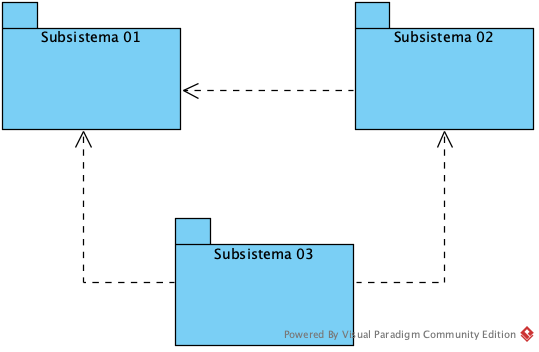
\includegraphics[width=.5\textwidth]{figuras/fig-subsistemas.png}
	\caption{Diagrama de Pacotes e os Subsistemas Identificados.}
	\label{fig-subsistemas}
\end{figure} 


% Tabela de subsistemas.
\begin{longtable}{|p{3cm}|p{12cm}|}
	\caption{Subsistemas identificados e suas interdependências.}
	\label{tbl-subsistemas} \\\hline 
	
	% Cabeçalho e repetição do mesmo em cada nova página. Manter como está.
	\rowcolor{lightgray}
	\textbf{Subsistema} & \textbf{Descrição} \\\hline		
	\endfirsthead
	\hline
	\rowcolor{lightgray}
	\textbf{Subsistema} & \textbf{Descrição} \\\hline		
	\endhead
	
	% Especificar os subsistemas abaixo, substituindo os exemplos.
	Subsistema 01 & Descrição do subsistema 01. \\\hline
	
	Subsistema 02 & Descrição do subsistema 02. \\\hline
	
	Subsistema 03 & Descrição do subsistema 03. \\\hline
\end{longtable}

